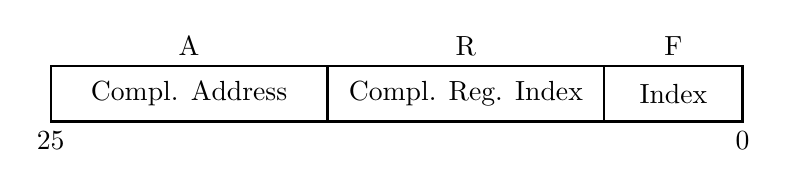
\begin{tikzpicture}[auto,thick,text badly centered]

	\begin{scope}[every node/.style={draw,rectangle,outer sep=0cm,minimum height=2em}]
		\node[minimum width=10.0em] (compl_a) {Compl. Address};
		\node[minimum width=10.0em] (compl_r) at (compl_a.east) [right] {Compl. Reg. Index};
		\node[minimum width=5.0em] (index) at (compl_r.east) [right] {Index};
	\end{scope}
	
	\node at (compl_a.north) [above] {A};
	\node at (compl_r.north) [above] {R};
	\node at (index.north) [above] {F};
	
	\node at (index.south east) [below] {0};
	\node at (compl_a.south west) [below] {25};
	
\end{tikzpicture}